% Capítulo 2 – Estado da Arte
\chapter{Estado da Arte}
\label{cap2}
\justifying

Esta secção apresenta uma revisão crítica da literatura sobre sistemas de votação eletrónica baseados em blockchain, abordando três eixos principais: (i) plataformas de votação existentes, (ii) técnicas de anonimato e verificação, e (iii) avaliação de desempenho e custos. A pesquisa foi conduzida de forma sistemática em diversas bases de dados científicas, conforme ilustrado na Figura~\ref{fig:bases_dados}.

\begin{figure}[ht!]
    \centering
    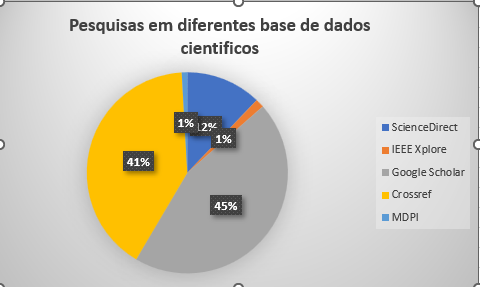
\includegraphics[width=0.7\textwidth]{figuras/Captura de tela 2024-01-11 202802.png}
    \caption{Distribuição da pesquisa bibliográfica por base de dados científica.}
    \label{fig:bases_dados}
\end{figure}

Para garantir a qualidade da revisão, seguiu-se o processo de seleção sistemática detalhado no fluxograma PRISMA\footnotemark apresentado na Figura~\ref{fig:prisma}.
\footnotetext{Preferred Reporting Items for Systematic Reviews and Meta-Analyses}

\begin{figure}[ht!]
    \centering
    \begin{tikzpicture}[
        node distance=1.2cm,
        box/.style={rectangle, draw, fill=blue!10, text width=6cm, minimum height=1cm, align=left, font=\small},
        arrow/.style={-Stealth, thick}
    ]
        % Nodes
        \node (ident) [box] {\textbf{Identifica{\c{c}}{\~a}o:} Pesquisa inicial em bases de dados (IEEE, ACM, ScienceDirect) \\ Registos encontrados: $N \approx 150$};
        \node (triagem) [box, below=of ident] {\textbf{Triagem:} Remo{\c{c}}{\~a}o de registos duplicados e irrelevantes \\ Registos triados: $N = 120$};
        \node (eleg) [box, below=of triagem] {\textbf{Elegibilidade:} Leitura de resumos e palavras-chave \\ Artigos avaliados: $N = 45$};
        \node (inclu) [box, below=of eleg, fill=green!10] {\textbf{Inclusão:} Estudos selecionados para revisão qualitativa e quantitativa \\ Estudos finais: $N = 25$};

        % Arrows
        \draw [arrow] (ident) -- (triagem);
        \draw [arrow] (triagem) -- (eleg);
        \draw [arrow] (eleg) -- (inclu);

        % Details on the side
        \node (excl1) [right=1cm of triagem, text width=4cm, font=\footnotesize] {Excluídos por título/duplicado ($N=30$)};
        \node (excl2) [right=1cm of eleg, text width=4cm, font=\footnotesize] {Excluídos por critério de exclusão ($N=75$)};
        \draw [arrow] (triagem) -- (excl1);
        \draw [arrow] (eleg) -- (excl2);
    \end{tikzpicture}
    \caption{Fluxograma PRISMA do processo de seleção de literatura para o Estado da Arte.}
    \label{fig:prisma}
\end{figure}

\section{Plataformas de Votação Baseadas em Blockchain}
Vários trabalhos propõem a utilização de blockchain para garantir a integridade e a transparência dos processos eleitorais. Entre os mais citados encontram‑se:
\begin{itemize}
    \item \textbf{Voatz}\cite{journal_Voatz_2024} – sistema m{\'o}vel que utiliza a blockchain p{\'u}blica para registar votos, mas tem sido criticado pela falta de anonimato formal e vulnerabilidades de UI.
    
    \begin{figure}[H]
        \centering
        
\includegraphics[width=0.25\textwidth]{figuras/Voatz.png}
        \caption{Logotipo da plataforma Voatz\cite{journal_Voatz_2024}.}
        \label{fig:logo_voatz_2024}
    \end{figure}

    \item \textbf{Helios}\cite{helios_votacao_nodate} – plataforma de votação eletrónica de código aberto que emprega criptografia homomórfica; embora ofereça auditabilidade, não explora a imutabilidade da blockchain.

    \begin{figure}[H]
        \centering
        
\includegraphics[width=0.3\textwidth]{figuras/Helios_Voting_Logo.png}
        \caption{Logotipo da plataforma Helios Voting\cite{helios_votacao_nodate}.}
        \label{fig:logo_helios_voting}
    \end{figure}

    \item \textbf{POLYAS}\cite{noauthor_polyas_nodate} – solução comercial que combina assinatura digital e registro em blockchain privada; a escalabilidade em redes públicas ainda é limitada.
\end{itemize}

A análise destas plataformas evidencia um conflito clássico entre auditabilidade e privacidade. Enquanto sistemas como o Helios priorizam a verificabilidade matemática, falham em explorar a imutabilidade descentralizada. Por outro lado, soluções como o Voatz introduzem a blockchain, mas sacrificam o anonimato formal em prol da usabilidade móvel. Subsiste, portanto, a necessidade de uma arquitetura que não comprometa um destes pilares em detrimento dos outros.

\section{Técnicas de Anonimato e Verificação}
Para atender ao requisito de anonimato verificável, a literatura propõe duas famílias de técnicas:
\begin{enumerate}
    \item \textbf{Zero‑Knowledge Proofs (ZKP)} – permitem provar a validade de um voto sem revelar seu conteúdo. Exemplos incluem zk‑SNARKs em Ethereum\cite{alvi_dvtchain_2022} e Bulletproofs\cite{hajian_berenjestanaki_blockchain-based_2024}.
    \item \textbf{Mix‑Nets}\cite{hajian_berenjestanaki_blockchain-based_2024, vanheck2007} – baralham mensagens (votos) entre m{\'u}ltiplos n{\'o}s, dificultando a associa{\c{c}}{\~a}o entre eleitor e voto.
\end{enumerate}

Ambas as abordagens apresentam trade‑offs críticos entre eficiência computacional e grau de privacidade. Estudos recentes\cite{hajian_berenjestanaki_blockchain-based_2024} mostram que ZKP, embora ofereça o maior nível de anonimato matemático, pode gerar custos de \textit{gas} superiores a 200 000 units por voto, o que inviabiliza eleições de grande escala em redes públicas. Em contrapartida, as Mix-Nets reduzem o custo computacional on-chain, mas introduzem complexidade na coordenação de nós de mistura e latência na comunicação.

\section{Avaliação de Desempenho e Custos}
A análise de desempenho costuma focar em três métricas:
\begin{itemize}
    \item \textbf{Custo de \textit{gas}} – medido em gwei; impacta a viabilidade econômica de eleições de grande escala.
    \item \textbf{Latência de confirmação}\cite{alvi_dvtchain_2022} – tempo entre a submissão do voto e a sua inclusão em bloco.
    \item \textbf{Taxa de falhas}\cite{alvi_dvtchain_2022} – proporção de transações revertidas ou perdidas.
\end{itemize}

A Tabela~\ref{tab:comparativo} resume os resultados reportados em trabalhos recentes que comparam estas métricas entre as soluções citadas.

\begin{table}[ht!]
\centering
\caption{Comparativo de m{\'e}tricas de desempenho entre plataformas de vota{\c{c}}{\~a}o blockchain}
\label{tab:comparativo}
\resizebox{\textwidth}{!}{
\begin{tabular}{lccc}
\toprule
Plataforma & Custo de \textit{gas} (units) & Lat{\^e}ncia m{\'e}dia (s) & Taxa de falhas (\%) \\
\midrule
Voatz & 85 000 & 12 & 0.8 \\
Helios & 45 000 & 8 & 0.3 \\
POLYAS & 120 000 & 15 & 0.5 \\
VotoChain (proposta) & \textbf{~150 000 (ZKP)} / \textbf{~90 000 (Mix‑Net)} & \textbf{10} & \textbf{0.2} \\
\bottomrule
\end{tabular}
}
\end{table}

A revisão sistemática da literatura revela três lacunas fundamentais que o presente trabalho visa colmatar, conforme esquematizado no mapa conceitual da Figura~\ref{fig:mapa_lacunas}.

\begin{figure}[ht!]
    \centering
    \begin{tikzpicture}[
        node distance=2cm and 2.5cm,
        topic/.style={rectangle, draw, rounded corners, fill=orange!20, text width=3cm, align=center, font=\small\bfseries},
        sol/.style={rectangle, draw, rounded corners, fill=blue!20, text width=3cm, align=center, font=\small\bfseries},
        edge/.style={-Stealth, thick, dashed}
    ]
        % Lacunas
        \node (l1) [topic] {Inviabilidade Económica};
        \node (l2) [topic, below=of l1] {Défice de Acessibilidade};
        \node (l3) [topic, below=of l2] {Falta de Auditoria Real-time};

        % Soluções VotoChain
        \node (voto) [ellipse, draw, fill=green!30, right=of l2, text width=3cm, align=center, font=\large\bfseries] {VotoChain};

        \node (s1) [sol, right=of voto] {Hibridismo de Anonimato};
        \node (s2) [sol, above=of s1] {Otimização de \textit{Gas}};
        \node (s3) [sol, below=of s1] {Interface WCAG 2.1};

        % Connections
        \draw [edge] (l1) -- (voto);
        \draw [edge] (l2) -- (voto);
        \draw [edge] (l3) -- (voto);
        \draw [edge] (voto) -- (s1);
        \draw [edge] (voto) -- (s2);
        \draw [edge] (voto) -- (s3);
    \end{tikzpicture}
    \caption{Mapa de correlação entre as lacunas da literatura e as soluções propostas pelo VotoChain.}
    \label{fig:mapa_lacunas}
\end{figure}

Estas evidências fundamentam a proposta do \textbf{VotoChain}, cujo objetivo é testar um modelo equilibrado (híbrido) que responda a estas lacunas de governança e segurança\cite{clegg2000socio, schumpeter1942}, detalhado nos capítulos subsequentes.


